\documentclass[hidelinks]{article}
\usepackage[utf8]{inputenc}
\usepackage[a4paper, total={7in, 10in}]{geometry}
\usepackage[dvipsnames]{xcolor}
\usepackage{amsmath}
\usepackage{tikz}
\usepackage{cite}
%\usepackage{tkz-euclide}
\usepackage[unicode]{hyperref}
\usepackage[all]{hypcap}
\usepackage{fancyvrb}
\usepackage{graphicx}
\usepackage{caption}
\usepackage{fvextra}

% Define a custom verbatim environment with white text 
\DefineVerbatimEnvironment{WhiteVerbatim}{Verbatim} {formatcom=\color{white}, fontsize=\small}

%\usetikzlibrary{angles,calc, decorations.pathreplacing}

\definecolor{carminered}{rgb}{1.0, 0.0, 0.22}
\definecolor{capri}{rgb}{0.0, 0.75, 1.0}
\definecolor{brightlavender}{rgb}{0.75, 0.58, 0.89}

\title{\textbf{CMPT 431 - Project}}
\author{Christopher M. Peer (Kit)}
\date{December 5th, 2024}

\begin{document}
\hypersetup{bookmarksnumbered=true,}
\pagecolor{black}
\color{white}
\maketitle

\section{Introduction}
\quad This project was created to compare the performance of thread parallel and distributed versions of the LocalPower Iteration Singular Value Decomposition algorithm to a standard serial Jacobi Singular Value Decomposition algorithm. The Local Power Iteration algorithm was invented by Li et al, it is outlined in the paper \cite{li2021communicationefficientdistributedsvdlocal}. A robust and fast method for extracting Singular Vectors from a matrix is useful for many methods in machine learning and data analysis, and any speedups from parallelizing this process would be a valuble pursuit in computation.
\newline
\quad LocalPower Iteration is an algorithm designed to find the $k^{th}$ largest Singular Vectors of an input matrix. LocalPower iteration parallelizes the task of Singular Value Decomposition by separating the matrix to be decomposed into equal sized sets of rows. Each processs/thread receives a set of matrix rows, then iteratively orthogonalises and transforms a set of output vectors into a set of Singular Vectors (Singularization) respective to the set of rows the process received from the matrix. Every $p$ iterations, the threads/processes collectively sum their output vectors; each thread/process's output vectors make a component of the Singular Vectors, the output vector sum makes the set of Singular Vectors of the whole matrix. Each thread/process then receives a copy of the summed output vectors and continues to iteratively "Singularize" them for $p$ iterations or until the program ends.
\newline 
\quad The computation time and error of the algorithm depends heavily on $p$ the number of iterations between communication stages: 
\begin{itemize} 
    \item With more iterations (larger $p$) between communication stages, there is less communication overhead and more "useful" computation, decreasing overhead
    \item With fewer iterations (smaller $p$) between communication stages, each process/thread generates it's set of Singular Vectors independently, creating more error.
    \item With more concurrent processing (threads/processes), the input matrix is split into smaller fragments, creating more specialised Singular Vectors in each thread / process, decreasing accuracy, but speeding up the computation time.
    \item With less concurrent processing (threads/processes), the input matrix is split into larger fragments, creating more generalised Singular Vectors in each thread / process, increasing accuracy, but slowing down computation time.
\end{itemize}
The intent behind designing the algorithm this way is to balance the tradeoff between Accuracy and Communication overhead by varying the number of iterations between communcation stages.

\section{Experimental Setup}
A serial version of LocalPower SVD is possible, but it is trivial since a serial program has no need to vary the number of iterations between communication stages because it doesn't need to communicate between threads/processes. A robust and fast alternative algorithm for serial computation is the JacobiSVD algorithm provided the Eigen Library \cite{eigen}, which provides a realistic standard in terms of speed and accuracy for a serial program. 
Each Singular Value Decomposition caluclation was done on the covertype dataset \cite{covertype_31}, a well conditioned dataset documenting tree coverage. 
\newline 
The LocalPower iteration algorithm was adapted for both distributed MPI and parallel threads versions. For each experiment, the algorithm was run for 16 total iterations to find the top 8 Singular Vectors of the input matrix, with variation on the number of iterations between communication stages, and variation on the number of concurrent processes/threads. With each combination of variables the experiment was run three times: total runtime, cumulative runtime of non-communication iterations, and error were recorded. Error and runtimes were averaged over all three runs.


\section{Computation Time}
The total computation time of Local Power iteration algorithm in these experiments is dependent on the number of iterations between communication stages (power iterations: $p$) and the number of threads/processes concurrently processing (nThreads: $n$)
It is important to note that during inter-thread/process communication stages, some useful computation takes place, but it is integral to the communication stage. Calculating the useful computation time does not take this into account and only calculate the iterations where no communication takes place. Although useful work is done during communication stages, the majority of time taken is up by communicating, so the additional useful time is not added. 

\subsection{Serial Computation}
Jacobi Singular Value Decomposition. This algorithm was run as a baseline to compare against the LocalPower algorithm. This algorithm was only implemented and run as serial a serial alternative to LocalPower as no direct serial version for LocalPower exists. This experiment was run using the JacobiSVD function provided by the Eigen library \cite{eigen}. The average runtime was: 
\begin{verbatim}
    Rank: 8
    Total time:28.594
    Error: 1.33759e-06
\end{verbatim}

\subsection{Parallel Computation}
The thread parallel algorithm of LocalPower was implemented using threads.cpp \cite{cppreference_thread} and Eigen \cite{eigen}. The variables in each experiment were: the number of iterations between communication stages (Power Iterations: $p$) and the number of concurrent processes (nThreads: $n$).Each variable was iterated over the range $p,n\in[2,4,8]$. For each combination of variables, the experiment was repeated 3 times and the results were averaged. The recorded metrics were: 
\begin{itemize}    
    \item The total computation time, from the moment the threads receive input, to the moment they return the Singular Vectors. 
    \item The cumulative computation time for all non-communication computations per each thread (All computations per thread that don't require communicating with other threads) 
\end{itemize}
The results are as follows:
\begin{figure}[h]
    \centering
    \begin{minipage}[h]{0.35\textwidth}
    \begin{WhiteVerbatim}
    p   n   Total Time          Thread Time	       
    8   8   12.496779           7.12853966666667
    4   8   12.558154           6.11907116666667
    2   8   12.509493           3.86968729166667
    8   4   12.1502836666667    7.092319	       
    4   4   12.44515            6.14964508333333
    2   4   12.639199           4.08572125	       
    8   2   12.6273286666667    7.53077983333333
    4   2   12.5934426666667    6.509494	       
    2   2   12.6201093333333    4.24881166666667
    \end{WhiteVerbatim}
    \end{minipage} 
    \hfill
    \begin{minipage}[h]{0.35\textwidth} 
        \centering 
        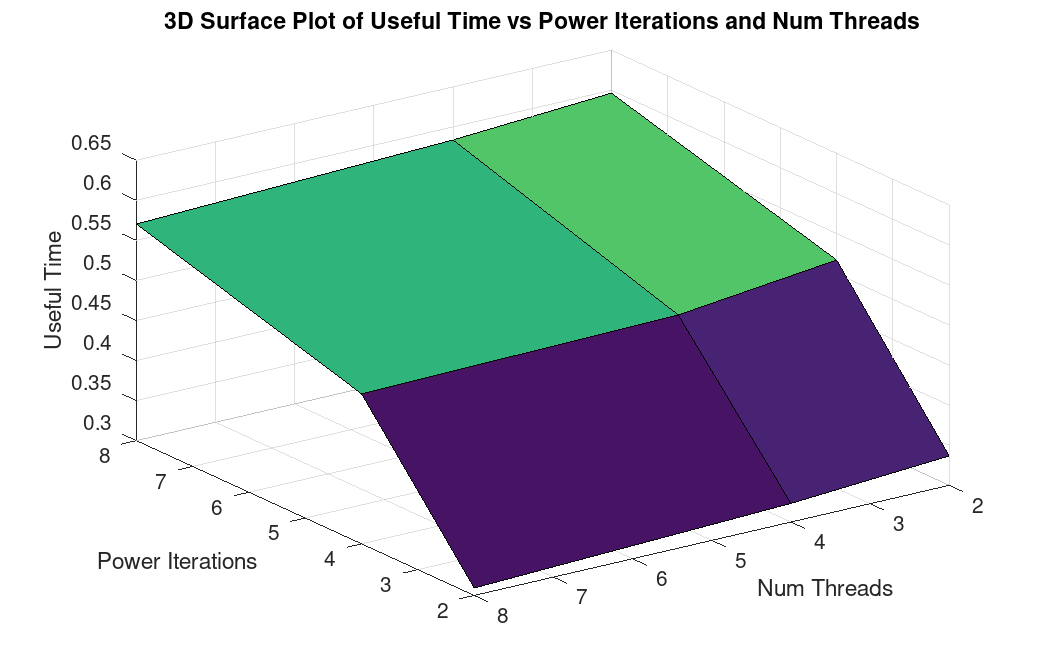
\includegraphics[width=\textwidth]{figures/useful_Time_parallel.png} 
        %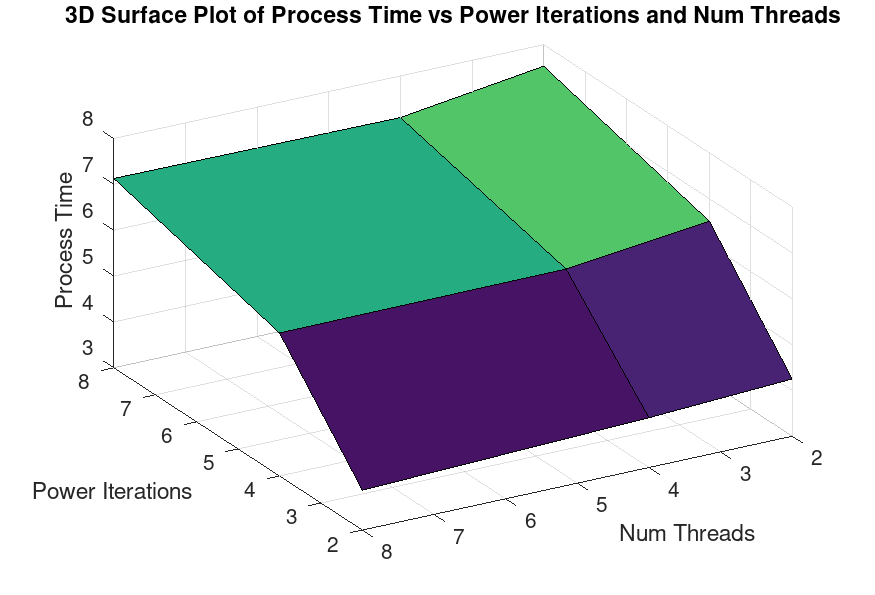
\includegraphics[width=\textwidth]{figures/p_time_parallel.png} 
        %\caption{figure}{Total Computation Time for Parallel Computation} 
    \end{minipage}
    \caption{lol}
\end{figure}
\newline
\quad The Ratio of useful time is the cumulative amount of non-communication time per thread, over the total time to compute. Useful Time = (Cumulative non-communication time)/(Total Time) .
\newline
From the graphic and the data above we can see the ratio of useful computation time increases with larger power iterations. With large power iterations the threads spend less time communicating and exchanging information and more time computing. It should be noted that the communication time between threads of a shared memory space is trivial compared to a distributed memory space. Total computation time would not change much with a change in the number of threads because communication between all threads is very quick. 

\newpage

\subsection{Distributed Computation}
\begin{figure}[h]
    \centering
    \begin{minipage}[h]{0.35\textwidth}
    \begin{WhiteVerbatim}
    p   n   Total Time          Process Time	       
    8   8   9.06261133333333    1.70064329166667
    4   8   8.605155            1.45637983333333
    2   8   8.14293933333333    0.979620791666667
    8   4   11.2341593333333    3.43791783333333
    4   4   10.6867413333333    2.92534958333333
    2   4   9.69740633333333    1.93053083333333
    8   2   14.9222093333333    6.8825485
    4   2   14.0515413333333    5.90270366666667
    2   2   12.219839           3.92319266666667
    \end{WhiteVerbatim}
    \end{minipage} 
    \hfill
    \begin{minipage}[h]{0.35\textwidth} 
        \centering 
        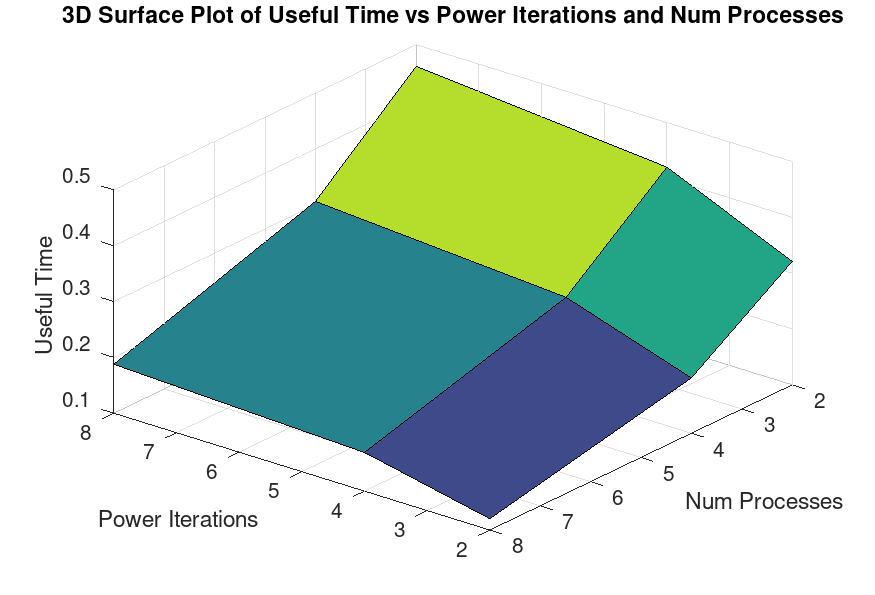
\includegraphics[width=\textwidth]{figures/useful_time_dist.png} 
        %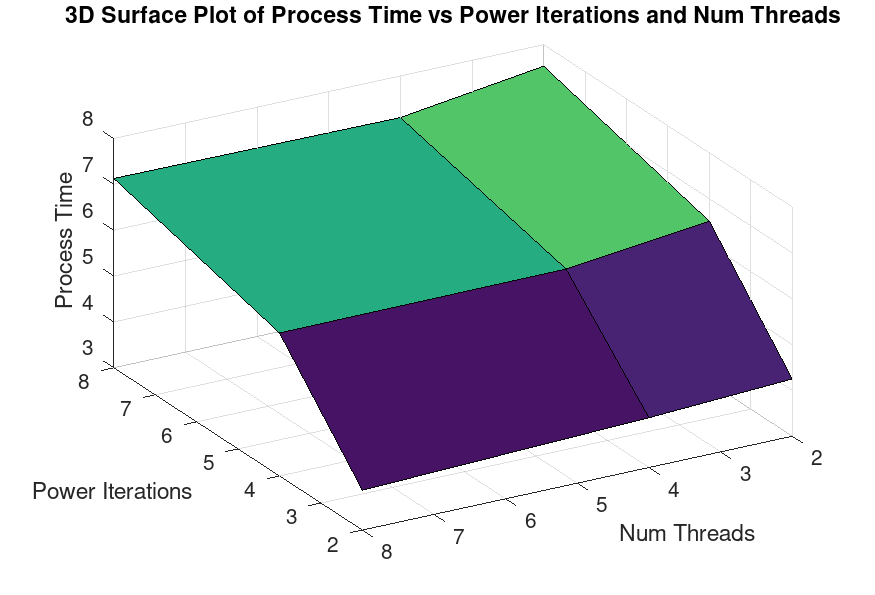
\includegraphics[width=\textwidth]{figures/p_time_parallel.png} 
        %\caption{figure}{Total Computation Time for Parallel Computation} 
    \end{minipage}
    \caption{lol}
\end{figure}

\quad The Ratio of useful time is the cumulative amount of non-communication time per thread, over the total time to compute. Useful Time = (Cumulative non-communication time)/(Total Time) .
\newline
From the graphic and the data above we can see both the power iterations and the number of concurrent processes are relevant the to amount of useful computation time. By increasing $p$ the number of iterations between communication stages, fewer communication stages are required, increasing the total amount of non-communication processing time and decreasing the time spent waiting for communications, which improves the Useful Time ratio. Decreasing the number of concurrent processes reduces the total amount of information to be communicated, and the number of sources/destinations to communicate with, making each communication stage less time costly. Even with only 2 processes, this method of computation can still acheive a significant reduction in total computation time compared to the baseline (JacobiSVD, 28.594 seconds), and spends a significant amount of that time computing rather than communicating. With greater numbers of threads and more communication stages the efficiency of this method degrades.

\section{Error} 

Both distributed and parallel version of this algorithm did not perform as well as the serial version as far as error. I suspect this may be due to to the implementation rather than the theoretical performance of the algorithm. The Gram-Schmidt orthogonalizer is not as accurate as other methods. This implementation also uses Sign-fixing as an alternative to the Orthogonal Procrustes Transformation (see the paper by Li et All) \cite{li2021communicationefficientdistributedsvdlocal} which is an $O(n)$ alternative to orthogonalizing on each communication stage, Sign-fixing is fast but lacks accuracy. Improvements to the implementation I provided may be able to improve the error, as well as using more iterations (Larger $t$) in total before finalising the output matrix. 


\subsection{Serial Computation}
Jacobi Singular Value Decomposition. This algorithm was run as a baseline to compare against the LocalPower algorithm. This algorithm was only implemented and run as serial a serial alternative to LocalPower as no direct serial version for LocalPower exists. This experiment was run using the JacobiSVD function provided by the Eigen library \cite{eigen}. The average error was: 
\begin{verbatim}
    Rank: 8
    Total time:28.594
    Error: 1.33759e-06
\end{verbatim}

\subsection{Parallel Computation}
\begin{figure}[h]
    \centering
    \begin{minipage}[h]{0.35\textwidth}
    \begin{WhiteVerbatim}
    p   n   Error
    8   8   3.580631
    4   8   3.17998366666667
    2   8   3.81608433333333
    8   4   4.53182166666667
    4   4   4.66895966666667
    2   4   4.28700566666667
    8   2   4.201654
    4   2   4.30027966666667
    2   2   4.42504833333333
    \end{WhiteVerbatim}
    \end{minipage} 
    \hfill
    \begin{minipage}[h]{0.35\textwidth} 
        \centering 
        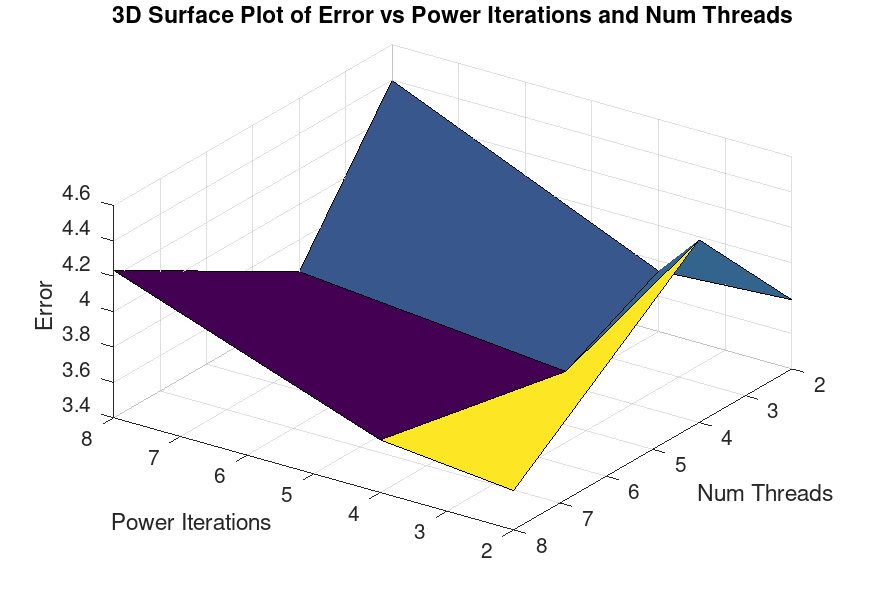
\includegraphics[width=\textwidth]{figures/Error_parallel.png} 
        %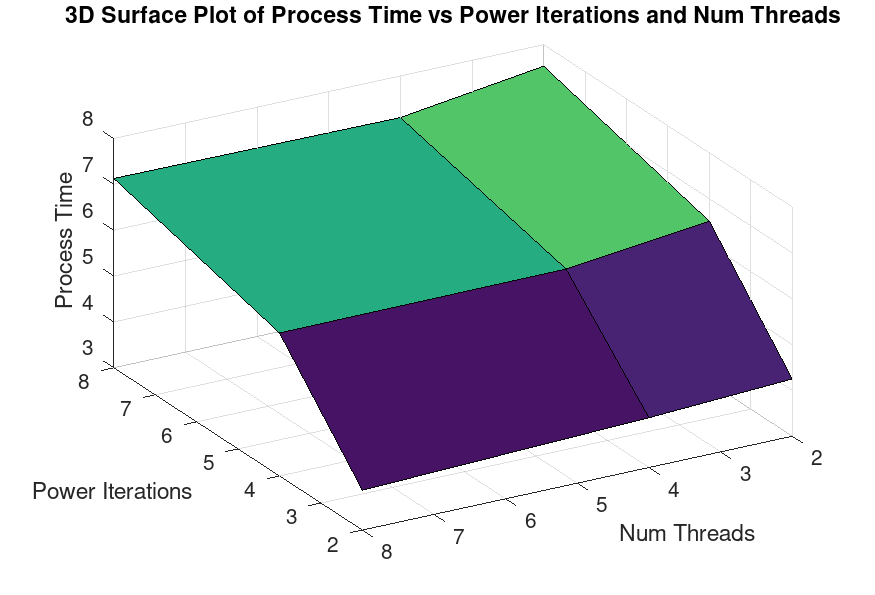
\includegraphics[width=\textwidth]{figures/p_time_parallel.png} 
        %\caption{figure}{Total Computation Time for Parallel Computation} 
    \end{minipage}
    \caption{lol}
\end{figure}

From the graphic and the data provided on the next page, we see error is dependent on both the number of concurrent threads and the number of Power iterations. Larger power iterations (greater $p$) meant there were fewer communication intervals over the entire computation, meaning each sub matrix was contributing more indivudually "singularized" vectors. With more concurrent processes (larger $n$) the original input matrix gets split into smaller pieces, decreasing the granularity of the problem. This had mixed effects on error over the distribution with respect to $p$.
\newpage
\subsection{Distributed Computation}
\begin{figure}[h]
    \centering
    \begin{minipage}[h]{0.35\textwidth}
    \begin{WhiteVerbatim}
    p   n   Error
    8   8   4.233081
    4   8   3.697486
    2   8   3.62206366666667
    8   4   3.61976
    4   4   3.47782166666667
    2   4   4.43357633333333
    8   2   4.39731933333333
    4   2   3.74245
    2   2   3.790614
    \end{WhiteVerbatim}
    \end{minipage} 
    \hfill
    \begin{minipage}[h]{0.35\textwidth} 
        \centering 
        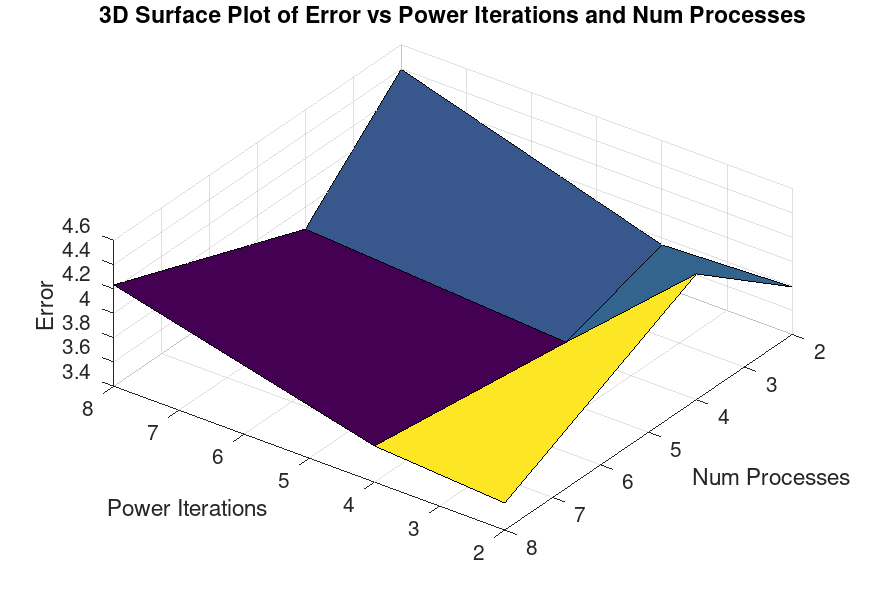
\includegraphics[width=\textwidth]{figures/Error_dist.png} 
        %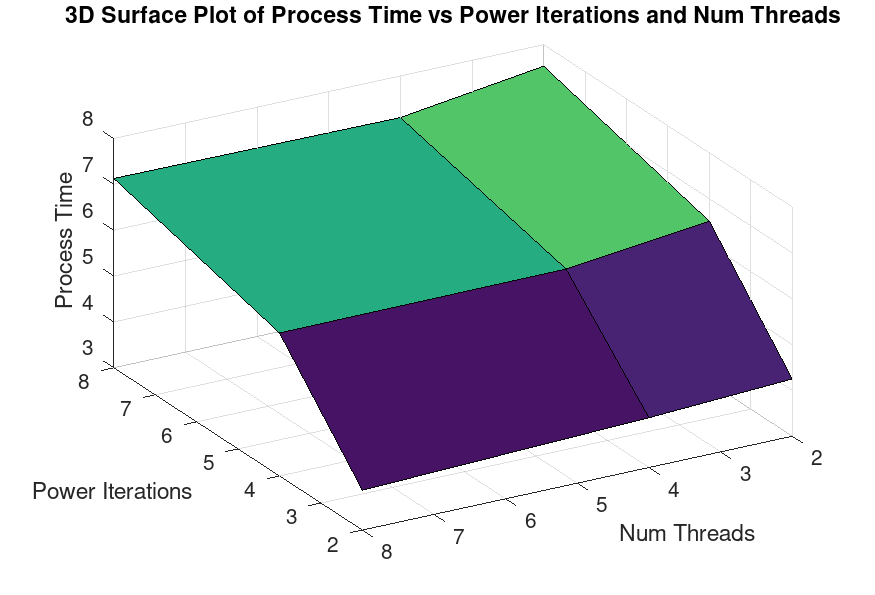
\includegraphics[width=\textwidth]{figures/p_time_parallel.png} 
        %\caption{figure}{Total Computation Time for Parallel Computation} 
    \end{minipage}
    \caption{lol}
\end{figure}

From the graphic and the data provided above, we see error is dependent on both the number of concurrent threads and the number of Power iterations. This is very similar to the results we see from the parallel process, although the distributed process has generally less error. Larger power iterations (greater $p$) meant there were fewer communication intervals over the entire computation, meaning each sub matrix was contributing more indivudually "singularized" vectors. With more concurrent processes (larger $n$) the original input matrix gets split into smaller pieces, decreasing the granularity of the problem. This had mixed effects on error over the distribution with respect to $p$.

\section {Discussion}
It is obivous that LocalPower iteration can has a dramatic improvement on speed: both decreasing the granularity of the problem by splitting the input matrix using concurrency, and varying communication efficiency to reduce the amount of communcation overhead during computation. I am happy with speed of the computation, but I want to improve the accuracy of this implementation. I suspect the large error in the results are because of a poorly implemented orthogonalizer. In future attempts I would improve this first, and then use larger total iterations to before producing an output. Improving the Sign-fixing method could also help improve the accuracy of the algorithm. In future I would also like to try this algorithm on poorly conditioned input data to see if that affects error, or input data with sparse sections.


\newpage

\bibliographystyle{plain} 
\bibliography{bibliolist}

\end{document}
